\par
\section{Driver programs for the {\tt Tree} object}
\label{section:Tree:drivers}
\par
%=======================================================================
\begin{enumerate}
%-----------------------------------------------------------------------
\item
\begin{verbatim}
drawTree msglvl msgFile inTreeFile inTagsFile outEPSfile
         heightflag coordflag radius bbox[4] frame[4] tagflag fontsize
\end{verbatim}
This driver program reads in a {\tt Tree} file and optionally a
tags {\tt IV} file and creates an EPS file with a simple
picture of a tree.
\par
\begin{itemize}
\item
The {\tt msglvl} parameter determines the amount of output.
\item
The {\tt msgFile} parameter determines the message file --- if {\tt
msgFile} is {\tt stdout}, then the output file is {\it stdout},
otherwise a file is opened with {\it append} status to receive any
output data.
\item
The {\tt inTreeFile} parameter is the input file for the {\tt Tree}
object. It must be of the form {\tt *.treef} or {\tt *.treeb}.
The {\tt Tree} object is read from the file via the
{\tt Tree\_readFromFile()} method.
\item
The {\tt inTagsFile} parameter is the input file for the {\tt IV}
vector object than holds the tags for the nodes. 
It must be of the form {\tt *.ivf} or {\tt *.ivb} or {\tt none}.
The {\tt IV} object is read from the file via the
{\tt IV\_readFromFile()} method.
\item
The {\tt outEPSfile} parameter is name of the
encapsulated Postscript file to be written.
\item
The {\tt heightflag} parameter is {\tt 'D'} to use a depth metric,
(i.e., parent and child are in adjacent levels),
and {\tt 'H'} to use a height metric (i.e., a leaf is on the
outermost level).
\item
The {\tt coordflag} parameter is {\tt 'C'} to put the tree in a
Cartesian coordinate system and {\tt 'P'} for a polar coordinate
system.
\item
The {\tt radius} parameter is the radius of each node in the tree.
\item
The {\tt bbox} parameter a sequence of four numbers that form the
bounding box: 
lower left $x$ value,
lower left $y$ value,
width and height.
\item
The {\tt frame} parameter a sequence of four numbers that form the
frame of the plot within the bounding box: 
lower left $x$ value,
lower left $y$ value,
width and height.
\item
When {\tt tagflag = 1}, tags are drawn on the nodes.
If {\tt tagsFile} is {\tt NULL}, then node ids will be drawn on the
nodes.
Otherwise, node ids will be taken from the {\tt tagsIV} object.
\item
The {\tt fontsize} parameter is the size of the font to be used to
draw the node labels.
\end{itemize}
Use the {\tt doDraw} script file as an example.
Four plots of a tree for the {\tt R2D100} matrix ordered by nested
dissection are found below.
%-----------------------------------------------------------------------
\end{enumerate}
\par
\begin{figure}[htbp]
\caption{{\sc R2D100}: domain/separator tree. 
         On the left {\tt heightflag = 'H'} and {\tt coordflag = 'C'},
         on the right {\tt heightflag = 'D'} and {\tt coordflag = 'C'}.}
\label{fig-R2D100-tree-HC}
\begin{center}
\mbox{
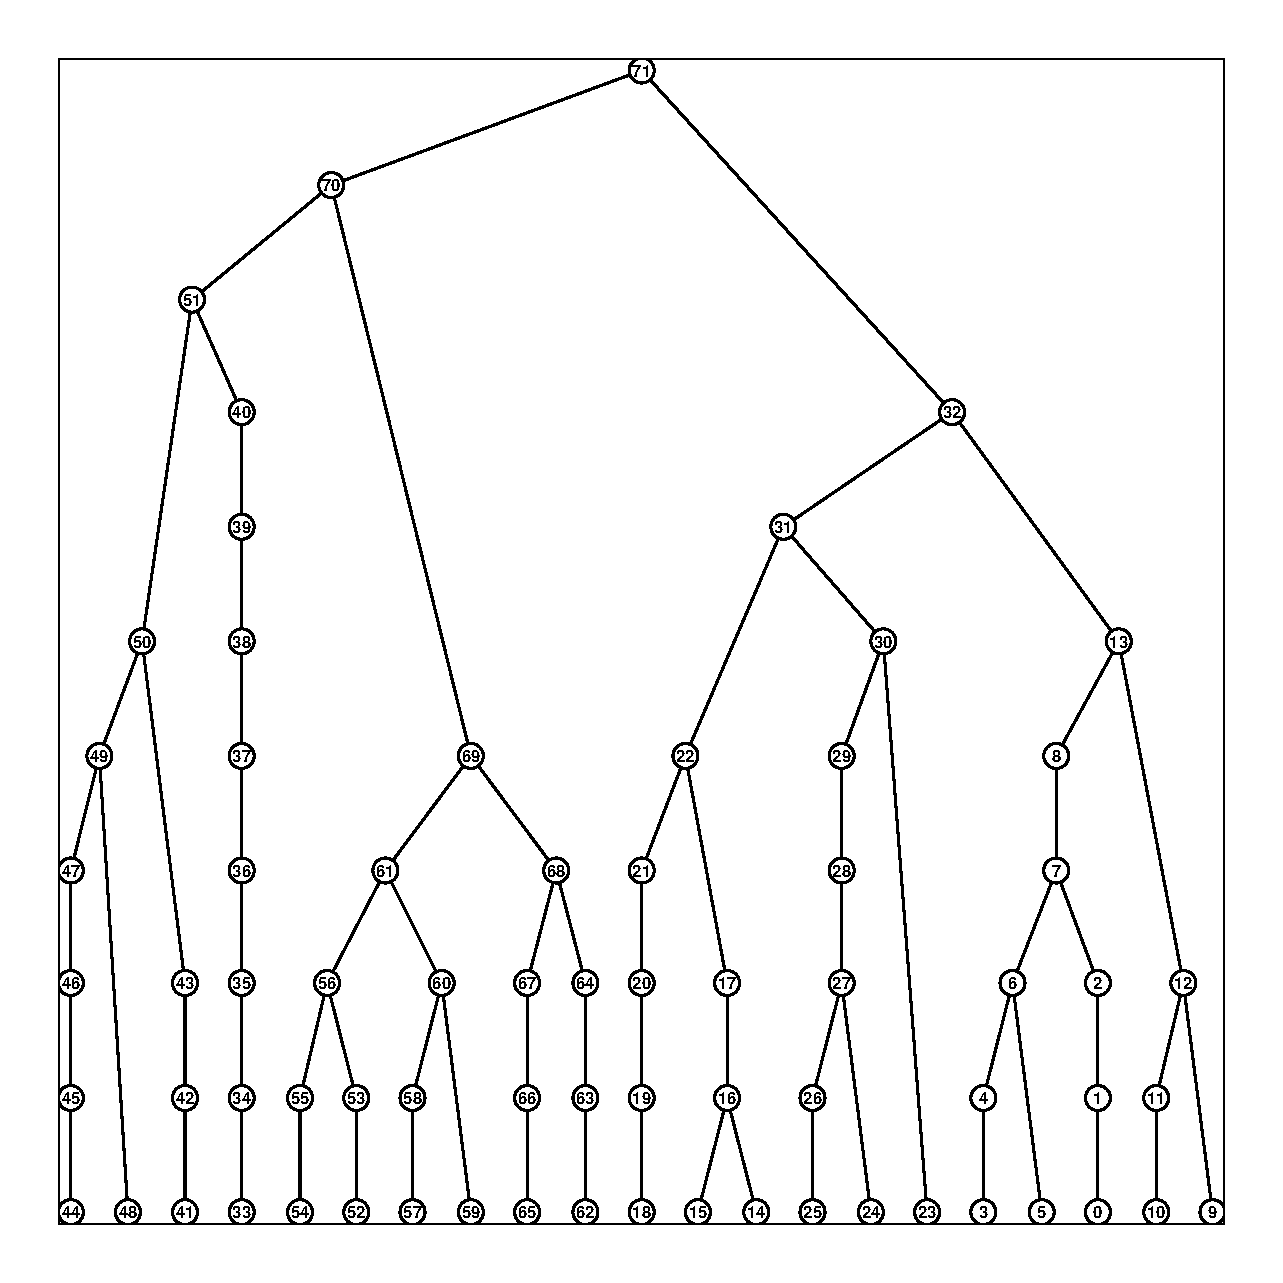
\psfig{file=../../Tree/doc/R2D100HC.eps,height=3.00in,width=3.00in}
}
\mbox{
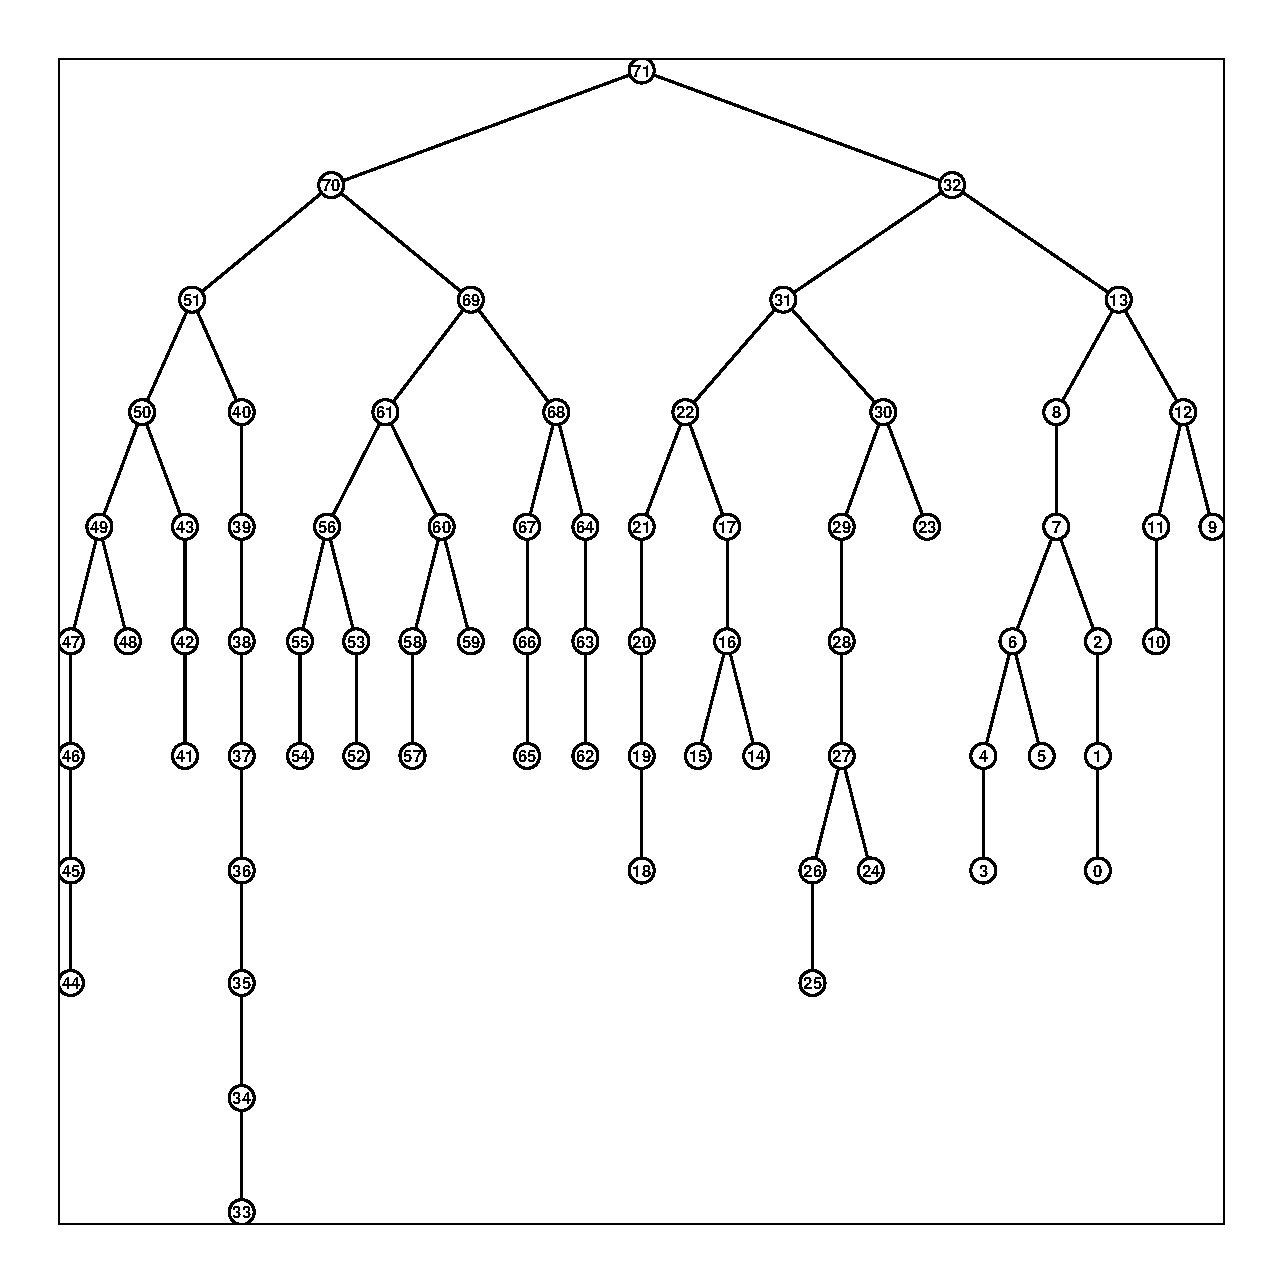
\psfig{file=../../Tree/doc/R2D100DC.eps,height=3.00in,width=3.00in}
}
\end{center}
\end{figure}
\par

\begin{figure}[htbp]
\caption{{\sc R2D100}: domain/separator tree. 
         On the left {\tt heightflag = 'H'} and {\tt coordflag = 'P'},
         on the right {\tt heightflag = 'D'} and {\tt coordflag = 'P'}.}
\label{fig-R2D100-tree-HP}
\begin{center}
\mbox{
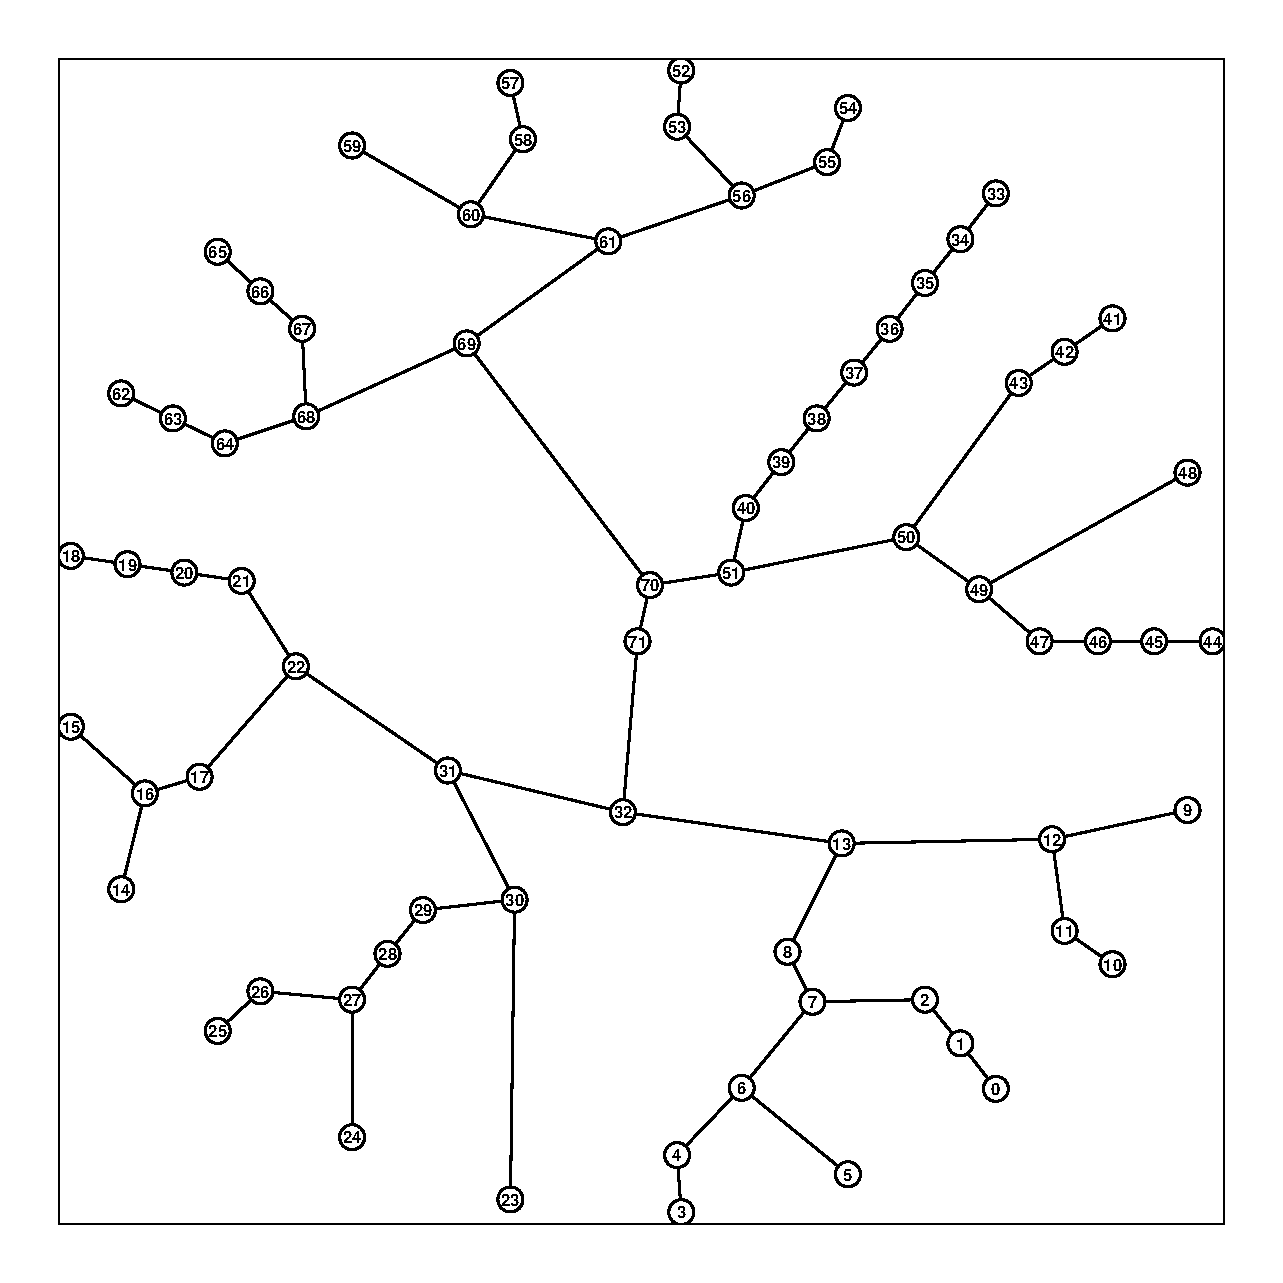
\psfig{file=../../Tree/doc/R2D100HP.eps,height=3.00in,width=3.00in}
}
\mbox{
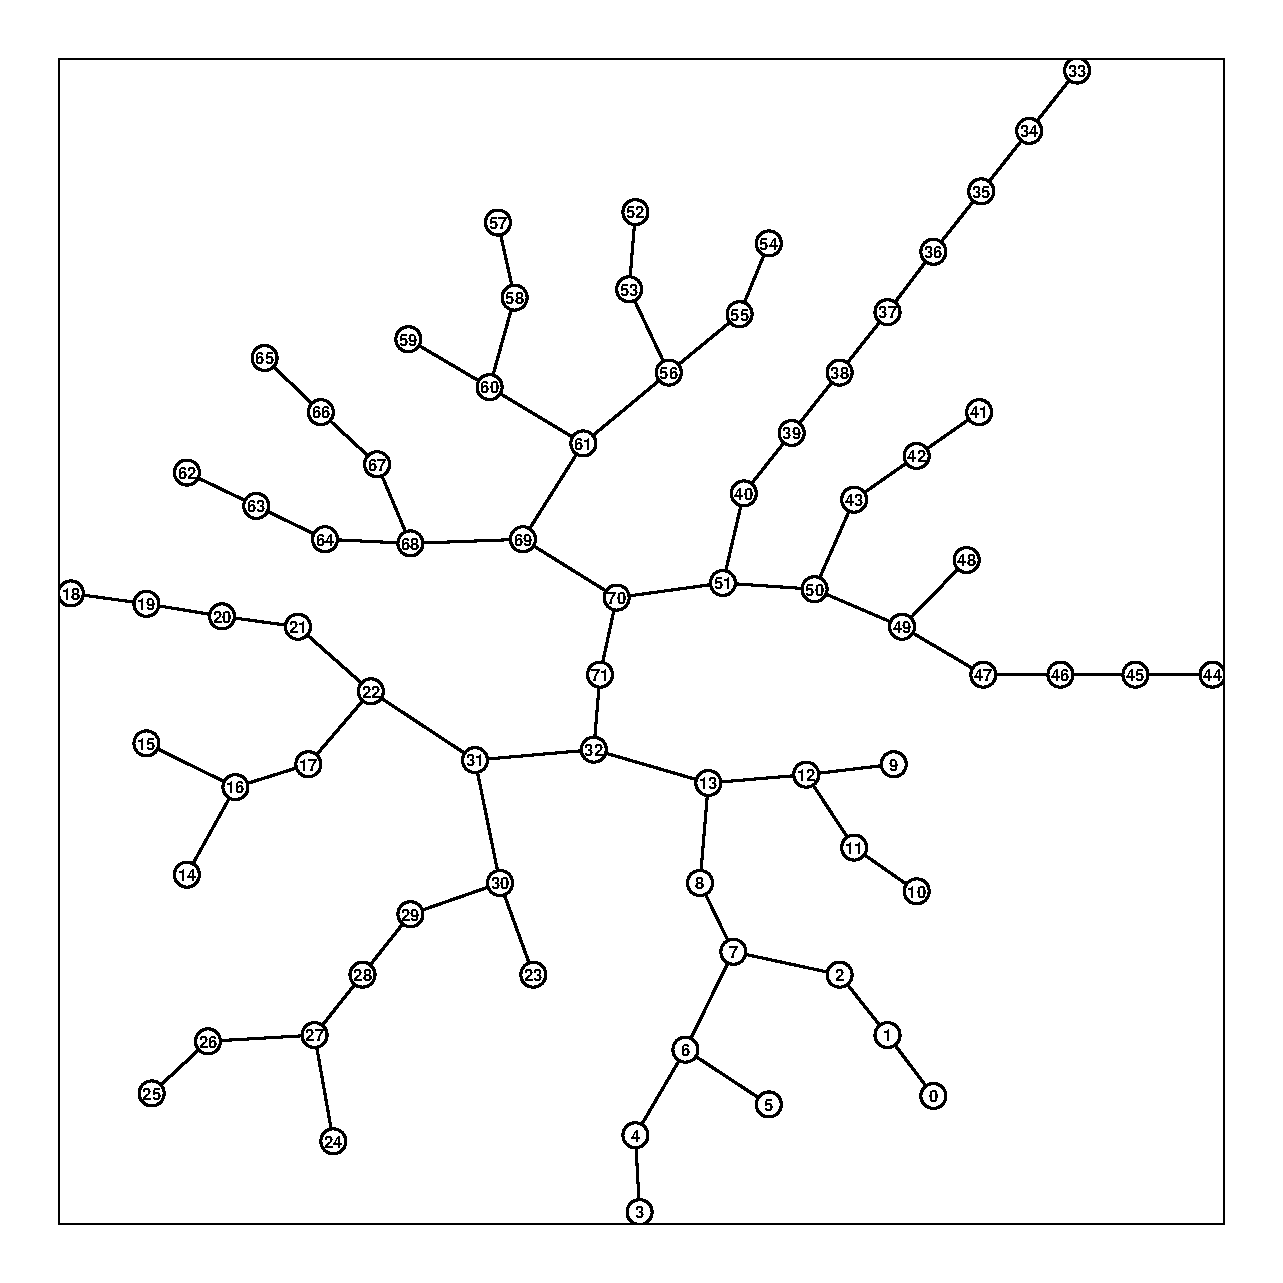
\psfig{file=../../Tree/doc/R2D100DP.eps,height=3.00in,width=3.00in}
}
\end{center}
\end{figure}

